\section{ Analysis of the application from architectural point of view}
In the requirements phase, earlier,was built an abstract model of the problem,which identifies what objects,entities,views are involved,how they relate to one another and how they look like.Probably now is the moment to describe the software architecture more thoroughly, from the implementation point of view,describing all the most important interfaces,classes, interaction between user and system and last but not least - the interaction between system components.In order to characterize the Spending Tracker application system, a collection of models were used:
\begin{itemize}
	\item \textbf{Use Case model}.It represents a set of use cases, actors, and their relationships.A use case represents a particular functionality of a system and it is used to describe the relationships among the functionalities and their controllers known also as \textbf{actors}.
	\item \textbf{Activity model}.It describes the flow of control in a system. It consists of activities and links.Activities are nothing but the functions of a system. Numbers of activity diagrams are prepared to capture the entire flow in a system.
	\item \textbf{Sequence model}.A sequence diagram is an interaction diagram.It is clear that the diagram deals with some sequences, which can be sequence of messages flowing from one object to another.
	\item \textbf{ Database model}.It represents a static structure diagram which underlines which are the entities where data are stored in the system,and the relationships which exist between them. \cite{UML}
\end{itemize}

This is the chapter where the Spending Tracker application is analysed using the above described diagrams.This will help to get a more clear image and a better understanding about the entire system and about the components interaction.

\subsection{Representation of the system via Use Case Diagrams}
The description of the system from the architectural point of view can be started from the Use Cases diagrams which presents the interaction of the user as an actor in the system.The first diagram represented in \ref{fig:firstusecase} describes all the possible actions a user can perform,a logged in user which is a prerequisite for all use cases diagrams.
\begin{figure}[H]
	\centering
	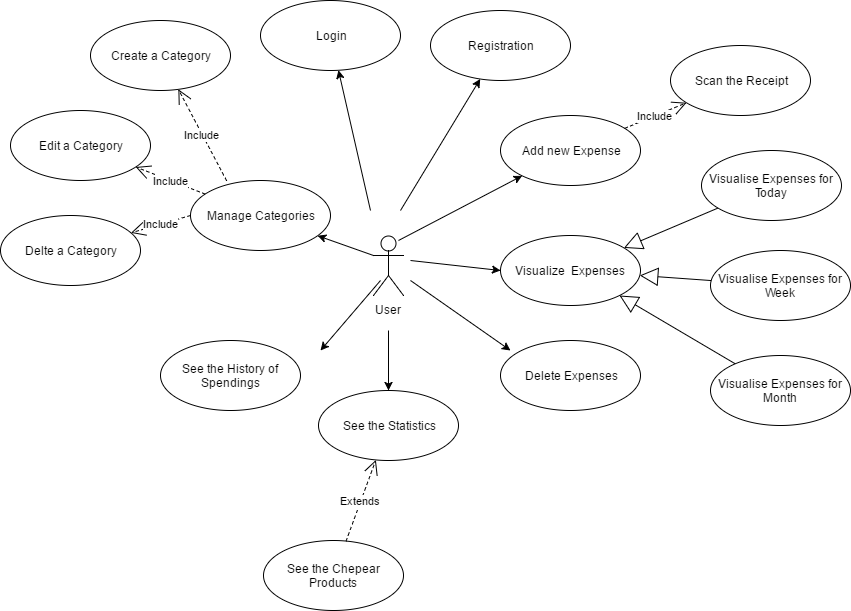
\includegraphics[width=18cm]{Chapter2/usecase1.png}
	\caption{Use case diagram for User}
	\label{fig:firstusecase}
\end{figure}
The primal activity of a user is login or registration activity in case the user installs the application for the first time. The next activity which should be performed before others is adding a new expense,an expense should be added in order to be able to perform all other activities as: 
Visualising expenses for today,for current week or for current month; deleting an expense; seeing the statistic which has an optional activity of seeing the cheaper products; or seeing the history of all expenses. Managing the categories represent another activity, it is independent and categories are predefined in the case of Spending Tracker application. They represents the existing stores in Chisinau.Categories can be created, edited and deleted as well.

The next diagram represent the activity of managing the categories.For accessing them, the left top spinner of the main page should be extended and Categories should be clicked from the list.See in \ref{fig:secondusecase} what activities can be performed on categories
\begin{figure}[H]
	\centering
	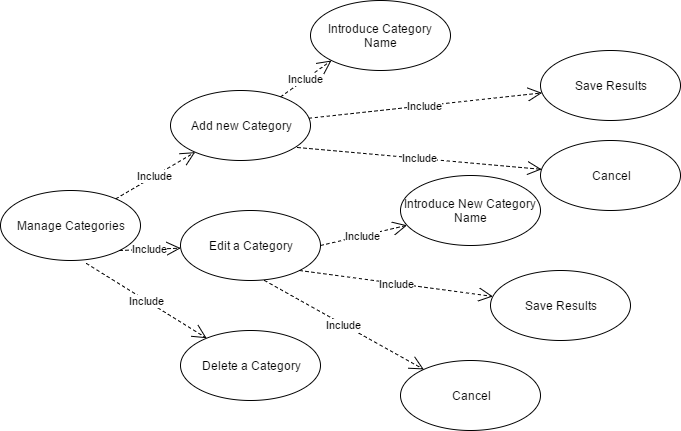
\includegraphics[width=18cm]{Chapter2/usecasecategoryng.png}
	\caption{Use case diagram for Categories}
	\label{fig:secondusecase}
\end{figure}
Managing categories are some very simple actions.Creating new category requires pressing the right bottom "plus" button which throws a window where is needed to introduce the category name,then the save button should be clicked or cancel in case of aborting the operation.The edit activity is almost the same,in the list of categories the desired category should be clicked and then a similar window is thrown as in case of creating a category, so the similar actions should be performed.For deleting a category is necessary keep pressing the desired category, after the selection the top right delete icon should be clicked.

The necessary activities to pe performed for registration process can be followed in the next \ref{fig:thirdusecase} .The process of registration is a typical one and it requires introducing of mandatory fields as  name,surname, password which have an optional control question case,also introducing of age and email are some mandatory action because they are used forward for performing some statistics according the expenses among different ages, email is used for sending a monthly report through it.Phone number is an optional field,it can be set in case the user want to receive a phone message according the monthly expenses.
\begin{figure}[H]
	\centering
	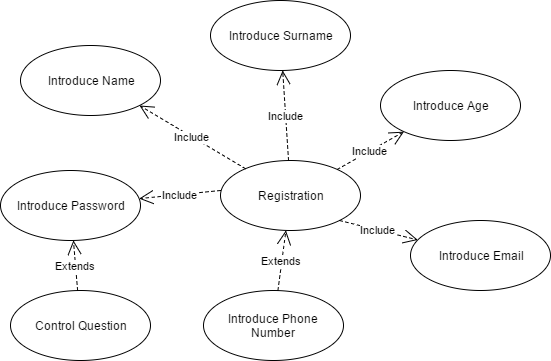
\includegraphics[width=18cm]{Chapter2/usecasereg.png}
	\caption{Use case diagram for Registration}
	\label{fig:thirdusecase}
\end{figure}

\subsection{System Analysis using Activity Diagrams}
Activity diagrams are those related to program flow and most often they are used for description of those business processes, they allow the functional thinking. 

Bellow in the figure \ref{fig:firstactivity} is represented the flow of steps to be done in order to perform the registration process.There are some typical steps for a registration process which are similar from one application to other.After introducing all necessary fields a process of checking the name,surname and password fields follows in order to confirm that such a user does not exists,then other mandatory fields are checked to confirm that they are filled with text.After all checking processes, data is approved or not, depending on information introduced.Once the information is approved data is stored in database and user is moved to the main application page.

\begin{figure}[H]
	\centering
	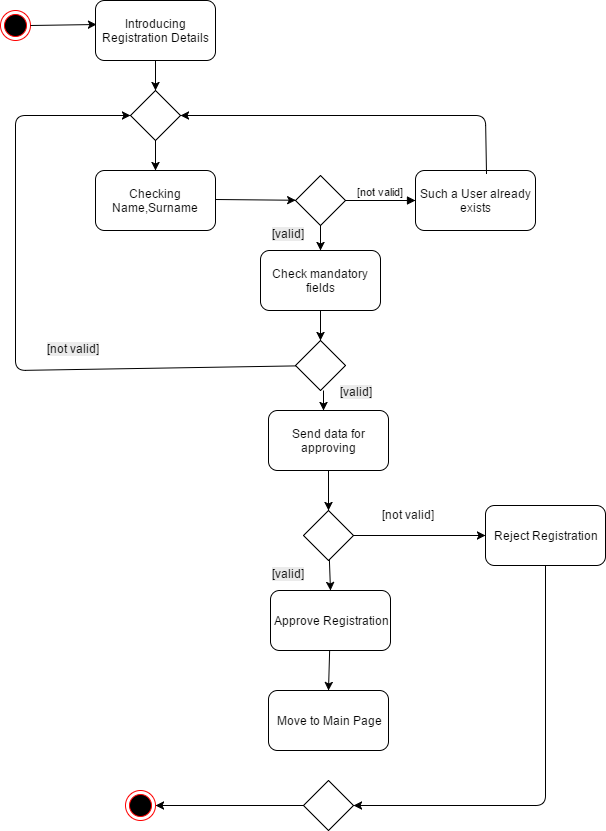
\includegraphics[width=18cm]{Chapter2/activityregistration.png}
	\caption{Activity diagram for Registration}
	\label{fig:firstactivity}
\end{figure}
\newpage
The next activity diagram represents the flow of scanning the receipt process.For adding new expense is necessary to scan the receipt by taking a photo of it, this actually is the primary functionality of the Spending Tracker application.First of all is necessary to go to the main page, where in bottom right corner the "plus" button is pressed which opens a new screen which the information about the process of scanning. The user is informed that is necessary to take a photo in order to scan the receipt.After pressing the button "Take a photo of your receipt", the android camera source is started and user must take a well focused photo of the receipt.After this follows a process of checking the recognized text,if text is not enough recognized the user must take a photo again.When results become valid, a category should be chosen in order to be able to save results to the database.
\begin{figure}[H]
	\centering
	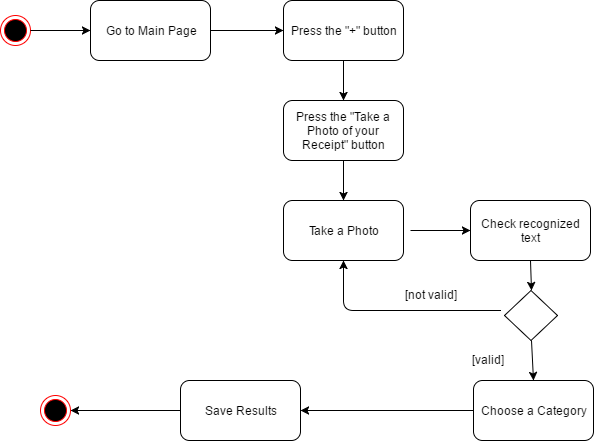
\includegraphics[width=18cm]{Chapter2/activityscan.png}
	\caption{Activity diagram for Scanning the Receipt}
	\label{fig:secondactivity}
\end{figure}

\subsection{Process interaction analysis using Sequence Diagram}
Sequence diagrams are that which emphasize the chronological course of exchanged information and this is exactly what is represented in next figure \ref{fig:firstsequence}.The process of adding a new expense is described using sequence diagram in more detailed form.All the participating objects are enumerated with their own life cycle and basically this diagrams are easier to be understand for developers and readers.  
\begin{figure}[H]
	\centering
	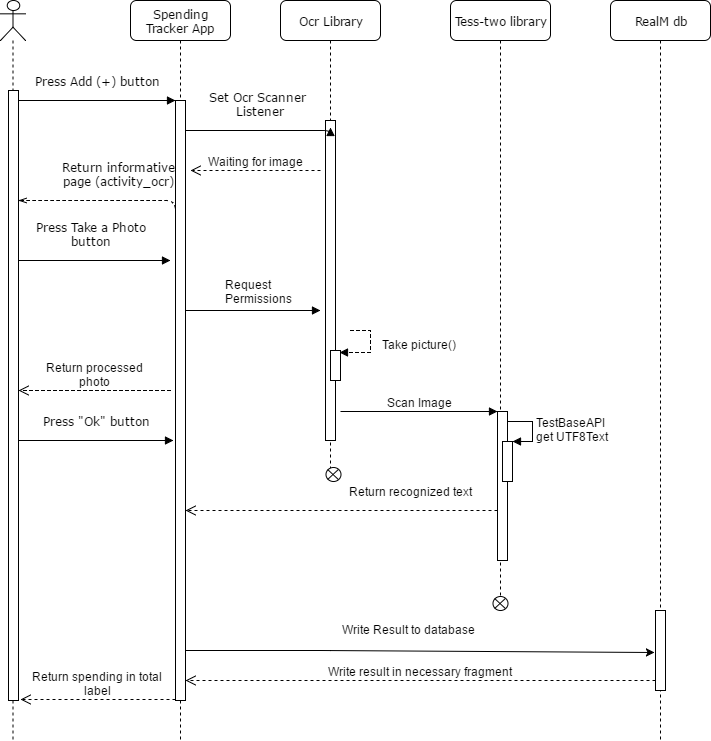
\includegraphics[width=18cm]{Chapter2/sequencescanreceipt.png}
	\caption{Activity diagram for Adding new Expense}
	\label{fig:firstsequence}
\end{figure}
The Spending Tracker application contains three basic packages: application, ocr library and tess-two library, last two used primarily for receipt text recognition.Database model is included in application package.The actor, which can be of a single type in the Spending Tracker application is the first primary entity in the system.
So, in order to add a new expense, user should press the "plus" right bottom corner on the main page of the application,at this moment the Ocr Scanner Listener is set and is waiting for an image and an informative page is returned to the user.The second page tells the user to press the next button "Take a photo of your receipt" in order to scan the receipt.This action requires the permission request which is done by Ocr library as well as taking photo action.After the photo was taken it is returned to the user.Then follows pressing the "Ok" button which suppose scanning the image itself, this step is performed by the Ocr library with the use of tess-two library, it contains the TextBaseAPI which is getting the text from the image and move it to a digital form.Recognized text is returned to the application after which the results are written to the database.Now the information is returned in necessary field in the application and user can visualise the scanned expense.
\subsection{The Database Model of the system}
\subsection{Final stage of product development: Deployment Diagram}